\section{Results}\label{sec:results}

\subsection{QBER Law}
Fig.~\ref{fig:qber} compares the simulated sifted-key QBER with \eqref{eq:qber} for $\ech\in\{0,0.02\}$ and $p\in[0,1]$, at $N=10^5$ and 60 trials per point. Agreement is within the statistical error bars (two standard deviations over trials), including the full-attack value $0.25$ at $\ech=0$ and $0.26$ at $\ech=0.02$. The $X$- and $Z$-basis error rates are statistically indistinguishable, as required by the symmetry argument in Lemma~\ref{lem:qber}. The figure also shows the asymptotic abort threshold, which an IR attack reaches at $p\approx0.39$ ($\ech=0$).

\begin{figure}[!t]
\centering
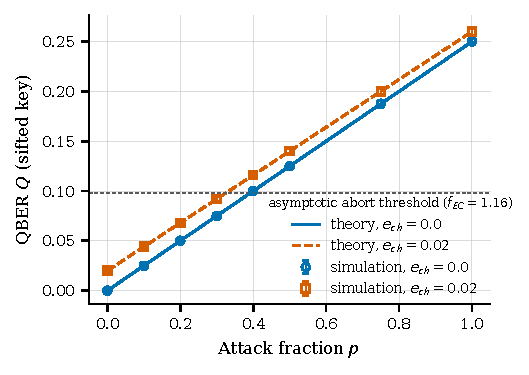
\includegraphics[width=\columnwidth]{figures/fig_qber.pdf}
\caption{Sifted-key QBER versus attack fraction $p$: theory \eqref{eq:qber} (lines) and Monte Carlo simulation (markers, $\pm2\sigma$ over trials).}
\label{fig:qber}
\end{figure}

\subsection{Key Rate versus Block Length}
Fig.~\ref{fig:rateN} shows $\ell/N$ as a function of $N$ for $\ech=0.01$ and four attack fractions, with the asymptotic limits~\eqref{eq:asym} as dotted lines. Without Eve, the first positive key appears near $N\approx5\times10^{3}$. The rate reaches $0.27$ bit/pulse at $N=10^5$, $0.45$ at $10^6$ and $0.68$ at $10^8$, against an asymptotic $0.83$. Attacks shift the whole curve to the right and flatten it: for $p=0.2$ no key exists below $N\approx4\times10^4$ and the rate is only $0.11$ bit/pulse at $N=10^6$.

\begin{figure}[!t]
\centering
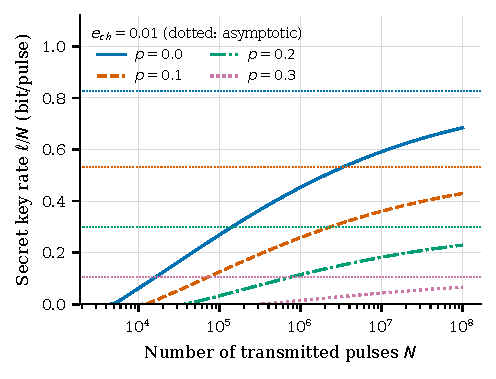
\includegraphics[width=\columnwidth]{figures/fig_rate_vs_N.pdf}
\caption{Secret-key rate versus the number of transmitted pulses for several attack fractions ($\ech=0.01$). Dotted lines: asymptotic rate \eqref{eq:asym}.}
\label{fig:rateN}
\end{figure}

Table~\ref{tab:mc} compares the full Monte Carlo protocol with the analytic prediction. The mean simulated rates agree with the analytic ones to within the trial-to-trial standard deviation in all cases, and to within $3\times10^{-4}$ bit/pulse for $N\ge10^5$. At $N=10^4$ the honest-abort probability is visible ($\approx0.3\%$), consistent with the design value of $z=3$ given the discreteness of the test statistic. At $N=10^4$ and $p\ge0.1$ the key length is non-positive, so the rate is zero by construction. The abort column for such zero-key cases reflects only the statistical test; the protocol would still terminate without key.

\begin{table}[!t]
\caption{Monte Carlo versus analytic key rate ($\ech=0.01$, $\epssec=10^{-10}$, $\epscor=10^{-15}$)}
\label{tab:mc}
\centering
\small
\begin{tabular}{@{}cccccc@{}}
\toprule
$N$ & $p$ & $q_X$ & abort (\%) & simulated $\ell/N$ & analytic \\
\midrule
$10^{4}$ & 0.0 & 0.61 & 0.27 & 0.0618 $\pm$ 0.0035 & 0.0620 \\
$10^{4}$ & 0.1 & 0.80 & 0.27 & 0.0000 $\pm$ 0.0000 & 0.0000 \\
$10^{4}$ & 0.2 & 0.80 & 0.13 & 0.0000 $\pm$ 0.0000 & 0.0000 \\
$10^{4}$ & 0.3 & 0.80 & 0.47 & 0.0000 $\pm$ 0.0000 & 0.0000 \\
$10^{5}$ & 0.0 & 0.77 & 0.00 & 0.2694 $\pm$ 0.0011 & 0.2694 \\
$10^{5}$ & 0.1 & 0.71 & 0.00 & 0.1257 $\pm$ 0.0006 & 0.1257 \\
$10^{5}$ & 0.2 & 0.61 & 0.00 & 0.0330 $\pm$ 0.0002 & 0.0330 \\
$10^{5}$ & 0.3 & 0.80 & 0.00 & 0.0000 $\pm$ 0.0000 & 0.0000 \\
$10^{6}$ & 0.0 & 0.87 & 0.00 & 0.4534 $\pm$ 0.0005 & 0.4537 \\
$10^{6}$ & 0.1 & 0.84 & 0.00 & 0.2585 $\pm$ 0.0003 & 0.2585 \\
$10^{6}$ & 0.2 & 0.79 & 0.00 & 0.1146 $\pm$ 0.0002 & 0.1147 \\
$10^{6}$ & 0.3 & 0.63 & 0.00 & 0.0148 $\pm$ 0.0000 & 0.0148 \\
\bottomrule
\end{tabular}
\end{table}


\subsection{Tolerable Attack Fraction}
Fig.~\ref{fig:ratep} shows how the key rate vanishes with growing $p$ for different $N$. Table~\ref{tab:pmax} lists $p_{\max}$. For $\ech=0.01$ the tolerated attack fraction is only $0.077$ at $N=10^4$, grows to $0.258$ at $N=10^5$, $0.326$ at $N=10^6$, and approaches the asymptotic value $0.360$ only at $N\approx10^{8}$. Increasing channel noise reduces $p_{\max}$ in all cases, because noise and IR errors share the same error budget; at $N=10^4$, $\ech=0.02$ leaves room for less than $4\%$ of intercepted pulses.

\begin{figure}[!t]
\centering
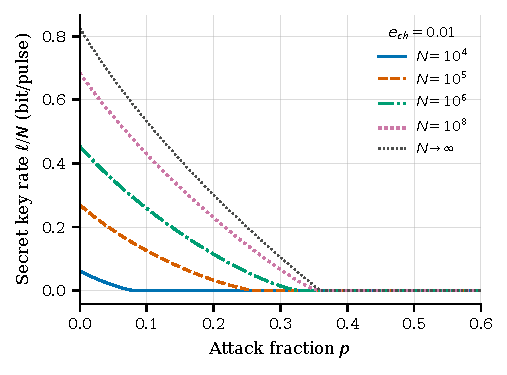
\includegraphics[width=\columnwidth]{figures/fig_rate_vs_p.pdf}
\caption{Secret-key rate versus attack fraction for several block lengths ($\ech=0.01$). The rate reaches zero at $p_{\max}(N)$.}
\label{fig:ratep}
\end{figure}

\begin{table}[!t]
\caption{Largest tolerable IR attack fraction $p_{\max}$ for a positive key}
\label{tab:pmax}
\centering
\small
\begin{tabular}{@{}cccccc@{}}
\toprule
$\ech$ & $N=10^4$ & $10^5$ & $10^6$ & $10^8$ & $N\to\infty$ \\
\midrule
0.00 & 0.116 & 0.293 & 0.360 & 0.389 & 0.392 \\
0.01 & 0.077 & 0.258 & 0.326 & 0.356 & 0.360 \\
0.02 & 0.037 & 0.222 & 0.292 & 0.322 & 0.325 \\
\bottomrule
\end{tabular}
\end{table}


\subsection{Effect of Channel Noise and Minimum Block Length}
Without an attacker, Fig.~\ref{fig:rateE} shows the key rate versus $\ech$. At $N=10^5$ the rate falls from $0.27$ bit/pulse at $\ech=0.01$ to zero near $\ech\approx 0.073$, whereas the asymptotic protocol tolerates $\ech\approx0.098$. Fig.~\ref{fig:nmin} gives the minimum block length. $\Nmin$ is about $2.6\times10^{3}$ at $Q=0$, $2.4\times10^4$ at $5\%$, $1.2\times10^5$ at $7.5\%$, $1.0\times10^6$ at $9\%$, and diverges at the asymptotic limit $Q^\ast$. For links with QBER above about $9\%$, block lengths above $10^6$ are required.

\begin{figure}[!t]
\centering
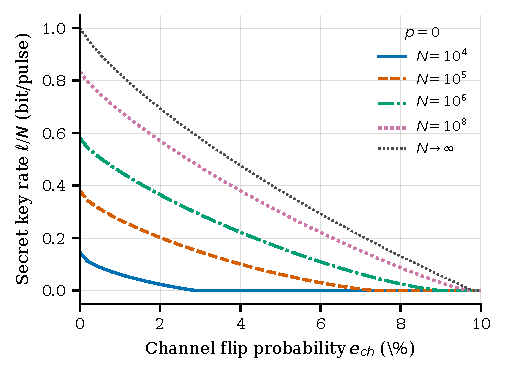
\includegraphics[width=\columnwidth]{figures/fig_rate_vs_e.pdf}
\caption{Secret-key rate versus channel flip probability without eavesdropper ($p=0$).}
\label{fig:rateE}
\end{figure}

\begin{figure}[!t]
\centering
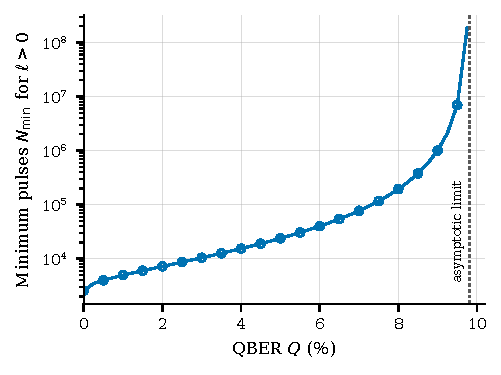
\includegraphics[width=\columnwidth]{figures/fig_nmin.pdf}
\caption{Minimum number of pulses for a positive key as a function of QBER (realised by IR attack with $\ech=0$, i.e.\ $Q=p/4$).}
\label{fig:nmin}
\end{figure}

\subsection{Empirical Validity of the Fluctuation Bound}
To check that \eqref{eq:serfling} is not violated, we sampled the total number of errors on a block of $n+k$ bits with $Q=0.03$, split it at random into a key part ($n$) and a test part ($k$), and estimated $\Pr[Q_n-Q_k\ge\gamma]$ from $4\times10^5$ trials. Table~\ref{tab:tail} shows that the empirical tails lie far below the bound, by at least one order of magnitude, so the bound is valid but conservative at these sizes. This is expected: the bound must hold for every possible $Q$ and for the worst-case distribution, whereas the test uses a single, favourable $Q$. The empirical test cannot probe the tiny probabilities ($\sim10^{-10}$) that the security parameter represents; it can only exclude gross violations.

\begin{table}[!t]
\caption{Empirical tail probability $\Pr[Q_n-Q_k\ge\gamma]$ versus bound \eqref{eq:serfling} ($Q=0.03$)}
\label{tab:tail}
\centering
\small
\begin{tabular}{@{}ccccc@{}}
\toprule
$n$ & $k$ & $\gamma$ & empirical & bound \\
\midrule
500 & 500 & 0.02 & 3.5e-02 & 9.1e-01 \\
500 & 500 & 0.04 & 1.5e-04 & 6.7e-01 \\
500 & 500 & 0.08 & 0.0e+00 & 2.0e-01 \\
2000 & 500 & 0.02 & 6.7e-03 & 8.5e-01 \\
2000 & 500 & 0.04 & 0.0e+00 & 5.3e-01 \\
2000 & 500 & 0.08 & 0.0e+00 & 7.8e-02 \\
5000 & 1000 & 0.02 & 1.4e-04 & 7.2e-01 \\
5000 & 1000 & 0.04 & 0.0e+00 & 2.6e-01 \\
5000 & 1000 & 0.08 & 0.0e+00 & 4.9e-03 \\
\bottomrule
\end{tabular}
\end{table}

